\section{Theorie}
\label{sec:Theorie}

%Allgemein
\subsection{Allgemein}
Trifft Licht auf einen Spalt oder ein kleines undurchlässiges Hinderniss, so weicht das Bild von den Gesetzen der geometrischen Optik ab.
Dies wird als Beugung des Lichtes bezeichnet.
Wird die Ausbreitung von Licht als klassische Welle beschrieben, so kann die Beugung erklärt werden.
Dabei wird der Teilchencharakter des Lichts vernachlässigt.

%Parallelspalt
\subsection{Beugung am Parallelspalt}
Um Beugung am Spalt zu Untersuchen wird entweder die Fresnelsche oder die Frauenhofersche Lichtbeugung verwendet.
Bei der Fresnelschen Näherung wird von einem geringen Abstand zwischen Lichtquelle - Spalt und Spalt - Beobachtungspunkt $P$ ausgegangen.
Also interferieren Lichtstrahlen im Punkt $P$.
\\
Ist die Lichtquelle weit vom Spalt entfernt, so kann die Frauenhofersche Näherung verwendet werden.
Es wird außerdem angenommen, dass sich der Beobachtungspunkt $P$ im unendlichen befindet.
Das hat zu folge, dass alle Strahlen die in $P$ interferieren unter den gleichen Winkel $\varphi$ gebeugt werden.
In Abb. \ref{fig:naeherung} ist die Fresnelsche und Frauenhofersche Beugung schematisch skizziert.
\begin{figure}
    \centering
    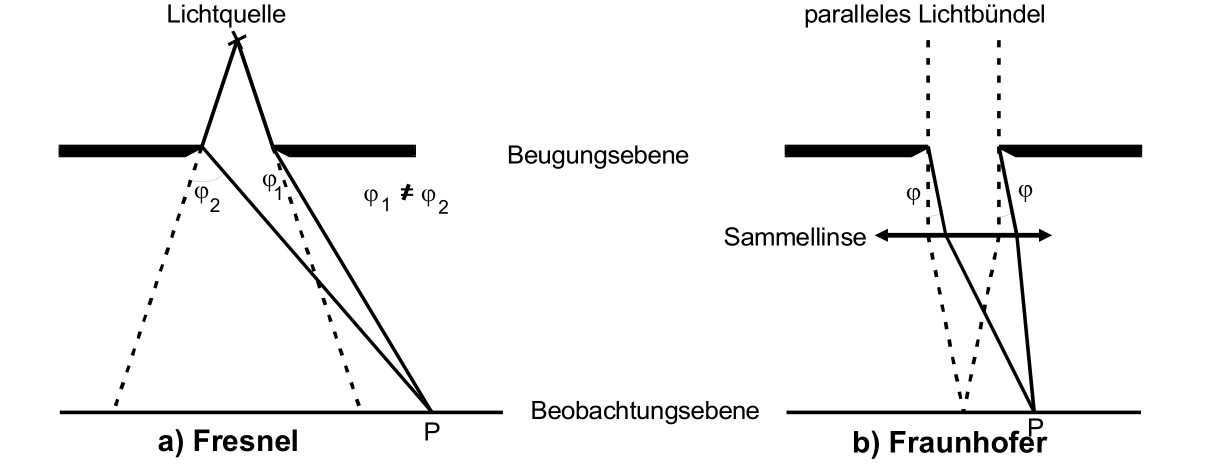
\includegraphics[width=0.8\textwidth]{content/data/naeherung.jpg}
    \caption{Die Fresnelsche (a) und Frauenhofersche Beugung (b) an einem Spalt. \cite[2]{anleitung}}
    \label{fig:naeherung}
\end{figure}
Ab hier wird nur die Frauenhofersche Beugung betrachtet.
Das erste Beugungsobjekt ist ein Spalt mit der Breite $b$ und einer Länge $l >> b$.
Das Licht wird also näherungsweise nur in einer Dimension begrenzt.
Die einfallende Welle hat die Feldstärke
\begin{equation*}
    A(z,t) = A_0 \cdot \mathrm{e}^{i(\omega t - \frac{2 \pi z}{\lambda})}
\end{equation*}
pro Längeneinheit der Wellenfront aus z-Richtung.
In dem Versuch wird als Lichtquelle ein Laser verwedet.
Die Entfernung zum Beobachtungspunkt $P$ ist groß zur Spaltbreite $b$.
\\
Das Huygenssche Prinzip besagt, dass jeder Punkt einer Wellenfront eine Elementarwelle aussendet.
Diese haben die Form einer Kugelwelle und interferieren miteinander und erzeugen eine neue Wellenfront.
Die Wellenfront entspricht der Einhüllenden der Elementarwellen.
Trifft Licht also durch den Spalt, so kann es sich nicht nur in die ursprüngliche Richtung ausbreiten, sondern sendet von jedem Punkt der Spaltöffnung eine Kugelwelle aus.
Zwei Strahlenbündel haben einen Phasenunterschied von
\begin{equation}
    \delta = \frac{2\pi x \sin (\varphi)}{\lambda} .
\end{equation}
Die Breite $x$ zwischen den Strahlenbündel sind infinitesimal klein und es kann über die gesamte Spaltbreite integriert werden:
\begin{align}
    B(z,t,\varphi) = A_0 \int_0^b \mathrm{e}^{i(\omega t - \frac{2 \pi z}{\lambda} + \delta)} \mathrm{d}x \\
   = A_0 \mathrm{e}^{i \left (\omega t - \frac{2 \pi z}{\lambda} \right )} \cdot \mathrm{e}^{\frac{\pi i b \sin \varphi}{\lambda}} \cdot \frac{\lambda}{\pi \sin \varphi} \cdot \sin \left (\frac{\pi b \sin \varphi}{\lambda} \right )
   \label{eqn:parallelspalt}
\end{align}
Die ersten beiden Exponentialfunktionen sind für die Intensitätsmessung unwichtig und Gleichung \eqref{eqn:parallelspalt} kann zu
\begin{equation}
    B(\varphi) = A_0 b \frac{\sin \mu}{\mu} \;\;\; \text{mit} \; \mu =\ \frac{\pi b \sin \varphi}{\lambda}
\end{equation}
vereinfacht werden.
Die Funktion ist in Abb. \ref{fig:funktion_parallel} dargestellt.
Die Nullstellen liegen bei $\sin \varphi_n = \pm n \frac{\lambda}{b} \; \text{für} \, n = 1, 2, ...$.
\begin{figure}
    \centering
    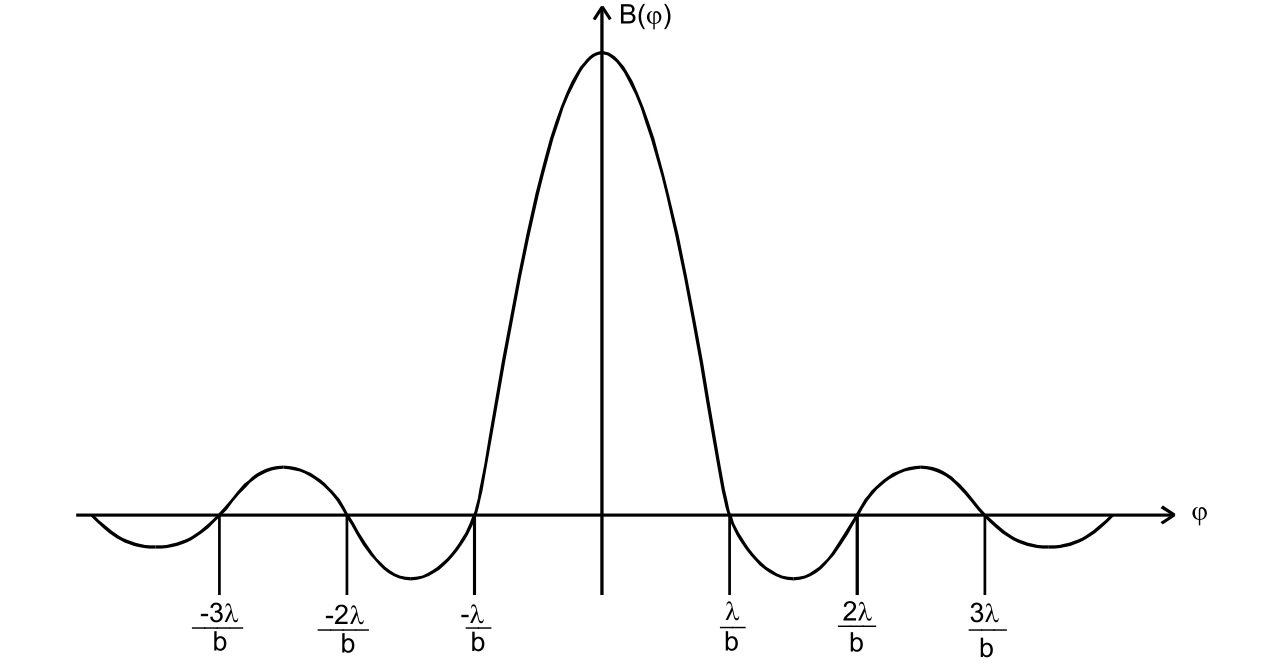
\includegraphics[width=0.8\textwidth]{content/data/funktion_parallel.jpg}
    \caption{Die Funktion \eqref{eqn:parallelspalt} der Amplitude an einem Parallelspalt gebeugten Ebenenwelle graphisch dargestellt. \cite[4]{anleitung}}
    \label{fig:funktion_parallel}
\end{figure}
Die Amplitude kann durch die hohe Lichtfrequenz nicht direkt gemessen werden.
Daher wird die zeitlich gemittelte Intensität mithilfe von
\begin{equation}
    I(\varphi) \propto B(\varphi)^2 = A^2_0 b^2 \left(\frac{\lambda}{\pi b \sin \varphi} \right)^2 \cdot \sin^2 \left ( \frac{\pi b \sin \varphi}{\lambda} \right )
    \label{eqn:beugungsfigur_parallel}
\end{equation}
ausgewertet.
Die Beugungsfigur \eqref{eqn:beugungsfigur_parallel} kann nicht negativ werden.
D.h. die Nulldurchgänge stellen die Minima dar.
Die dazwischenliegenden Maxima nehmen mit dem Quadrat des Beugungswinkel ab.

%Doppelspalt
\subsection{Beugung am Doppelspalt}
Fällt Licht durch einen Doppelspalt (siehe Abb. \ref{fig:doppelspalt}), so kann die Beugungsverteilung als Überlagerung zweier Einfachspalte mit der Breite $b$ und dem Abstand $s$ behandelt werden.
\begin{figure}
    \centering
    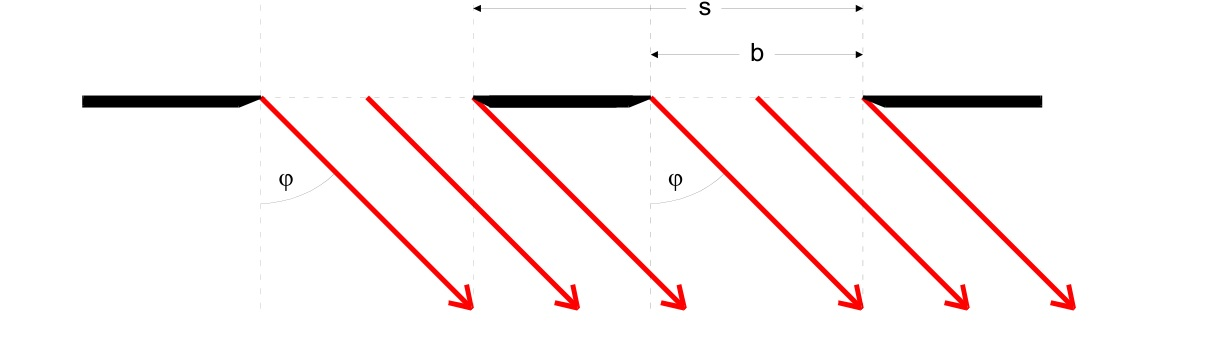
\includegraphics[width=0.8\textwidth]{content/data/doppelspalt.jpg}
    \caption{Beugung an einem Doppelspalt schematisch dargestellt. \cite[5]{anleitung}}
    \label{fig:doppelspalt}
\end{figure}
Die Intensitätsverteilung des Beugungsbildes ist durch
\begin{equation}
    I(\varphi) \propto B(\varphi)^2 = 4 \cdot \cos^2 \left( \frac{\pi s \sin \varphi}{\lambda} \right) \cdot \left( \frac{\lambda}{\pi b \sin \varphi} \right)^2 \cdot \sin^2 \left ( \frac{\pi b \sin \varphi}{\lambda} \right )
    \label{eqn:beugungsfigur_doppel}
\end{equation}
gegeben.
Die Funktion der Beugungsfigur setzt sich aus der Beugungsfigur eines Einfachspalts und einem $\cos^2$-Term zusammen.
Zusätzlich zu den Nullstellen des Einfachspalts existieren weitere Intensitätsminima:
\begin{equation*}
    \varphi(k) = \arcsin \left( \frac{2k+1}{2s} \right) \cdot \lambda \;\;\; \text{mit} \;\; k = 0, 1, 2, ...
\end{equation*}

%Fraunhofersche Beugung, Fourier
\subsection{Frauenhofersche Beugung und Fourier-Transformation}
Das Beugungsbild $B(\varphi)$ \eqref{eqn:beugungsfigur_doppel} kann als Fourier-Transformierte der einfallenden Welle interpretiert werden.
Die Fouriertransformation ist allgemein wie folgt definiert:
\begin{equation}
    g(\xi) = \int_{-\infty}^\infty f(x) \mathrm{e}^{i x \xi} \mathrm{d}x
    \label{eqn:fourier}
\end{equation}
Die Apertfunktion $f(x)$ beschreibt die Gestalt des Spalts und hat hier die Form
\begin{equation}
    f(x) = \left \{ \begin{array}{ll} A_0, & 0 \leq x \leq b \\
    0, & \text{sonst}\end{array} \right. .
    \label{eqn:aperfunktion}
\end{equation}
Nach einsetzen der Apertfunktion \eqref{eqn:aperfunktion} in die Fouriertransformation \eqref{eqn:fourier} und anschließendem umformen, ergibt sich
\begin{equation}
    g(\xi) = \frac{2 A_0}{\xi} \mathrm{e}^\frac{i \xi b}{2} \cdot \sin \left( \frac{\xi b}{2} \right) .
    \label{eqn:fourier_erg}
\end{equation}
Wird 
\begin{equation*}
    \xi = \frac{2\pi \sin \varphi}{\lambda}
\end{equation*}
gesetzt, so ergibt sich die zuvor berrechnete Beugungsfigur \eqref{eqn:parallelspalt}.
Das Huygenssche Prinzip wird als durch die Fouriertransformation mathematisch beschrieben.
Die Fouriertransformation ist rückführbar, daher kann aus der Amplitudenfunktion die Gestalt des beugenden Objektes $f(x)$ ermittelt werden.